\documentclass[11pt]{article}

\usepackage[font=small,format=plain,labelfont=bf,textfont=it]{caption}


\usepackage[colorlinks]{hyperref}
\usepackage[svgnames]{xcolor}

\usepackage{todonotes}



\hypersetup{    
	citecolor=DarkBlue,
	bookmarksnumbered=true,
	urlcolor=Indigo,linkcolor=DarkBlue
}



\usepackage{aliascnt} 
\usepackage{fullpage, verbatim, amsfonts, amsmath, amssymb, amsthm, latexsym, setspace, graphicx}
\usepackage[T1]{fontenc}
\usepackage[latin9]{inputenc}
\usepackage{geometry}
\usepackage{color}
\usepackage{natbib}
\usepackage{dsfont}

\usepackage{subfigure}



\usepackage{setspace}
\onehalfspacing


\usepackage{tikz}
\usetikzlibrary{patterns}




\geometry{verbose,letterpaper,lmargin=1in,rmargin=1in, top = 1in, bottom = 1.2in}

\newtheorem*{thmbw}{Blackwell's Theorem}

\theoremstyle{plain}
\newtheorem{thm}{Theorem}

\newtheorem{lem}{Lemma}

\newtheorem{prop}{Proposition}

\newtheorem{cor}{Corollary}

\newtheorem{defn}{Definition}
\newtheorem{claim}{Claim}
\newtheorem*{obs}{Observation}
\newtheorem{ex}{Example}
\newtheorem{assume}[thm]{Assumption}
\newtheorem{axiom}[thm]{Axiom}


\theoremstyle{remark}
\newtheorem*{rem}{Remark}

\def\subsectionautorefname{Section}
\def\exampleautorefname{Example}
\def\thmautorefname{Theorem}
\def\propautorefname{Proposition}
\def\lemautorefname{Lemma}
\def\exautorefname{Example}
\def\conditionautorefname{Condition}
\def\equationautorefname{Equation}
\def\propertyautorefname{Property}
\def\sectionautorefname{Section}
\let\subsectionautorefname\sectionautorefname
\let\subsubsectionautorefname\sectionautorefname
\def\assumptionautorefname{Assumption}
\def\inequalityautorefname{Inequality}
\def\figureautorefname{Figure}
\def\assumptionautorefname{Assumption}
\def\claimautorefname{Claim}
\def\corautorefname{Corollary}


\newcommand{\bu}{\mathbf{u}}
\newcommand{\bb}{\mathbf{b}}
\newcommand{\bm}{\mathbf{m}}
\newcommand{\bd}{{\boldsymbol\delta}}

\newcommand{\po}{\mathcal{H}}


\begin{document}
 
\title{Robust Merging of Information\footnote{We are grateful to Nageeb Ali, Marc Henry, Jiangtao Li, Elliot Lipnowski, Pietro Ortoleva, and Shamim Sinnar for valuable comments.}


}
\author{Henrique de Oliveira\thanks{S\~{a}o Paulo School of Economics - FGV. Email: \href{mailto:henrique.oliveira@fgv.br}{henrique.oliveira@fgv.br} }  \and Yuhta Ishii\thanks{ Pennsylvania State University. Email: \href{mailto:yxi5014@psu.edu}{yxi5014@psu.edu} } \and Xiao Lin\thanks{  Pennsylvania State University. Email: \href{mailto:xiao@psu.edu}{xiao@psu.edu} } 
}
\date{\today}

\maketitle


\abstract{
When multiple sources of information are available, any decision must take into account their correlation. If information about this correlation is lacking, an agent may find it desirable to make a decision that is robust to possible correlations. Our main results characterize the strategies that are robust to possible hidden correlations. In particular, with two states and two actions, the robustly optimal strategy pays attention to a single information source, ignoring all others. More generally, the robustly optimal strategy may need to combine multiple information sources, but can be constructed quite simply by using a decomposition of the original problem into separate decision problems, each requiring attention to only one information source. An  implication is that an information source generates value to the agent if and only if it is best for at least one of these decomposed problems.
}
	
%\newpage
%\listoftodos

\newpage

\section{Introduction}
During the COVID-19 pandemic, testing has been essential in effectively monitoring the transmission of the virus. Two prevalent diagnostic tests are the molecular and antigen tests, which differ in checking the virus's genetic materials or specific proteins.\footnote{For more information regarding these tests, see for example \url{https://www.fda.gov/health-professionals/closer-look-covid-19-diagnostic-testing}.}  It might then be appealing to use both tests.\footnote{Taking both tests is indeed recommended by FDA: ``(for antigen test) positive results are usually highly accurate, \dots negative results may need to be confirmed with a molecular test.'' Some medical providers always require one to take both tests.} However, in order to correctly interpret the joint pair of results from the two tests, knowledge of their correlation is crucial. For example, conditional on the molecular test producing a false negative, what is the probability that the antigen test also yields a false negative? Although the likelihoods of false positives and false negatives for each test are  well-understood, data regarding the correlations between these tests is scarce.\footnote{See for example \citet{dinnes2020rapid}.} With such limited information about these correlations, how is a
health authority supposed to make use of the results of both tests?

Such unclear correlation between information sources is a common difficulty in practical decision problems. For example, someone might have access to the opinions of multiple experts (such as doctors), but these experts might use similar specialized sources (such as a flawed study). In this paper, we assume that the agent fully understands each information source in isolation, but has no knowledge about the correlations between different information sources. We then look for strategies that are robust to such correlation, by considering the worst possible correlation that could occur. 

Our main results characterize robustly optimal strategies. The simplest characterization occurs when we have two states and two actions. In that case, to guard against hidden correlation, one must resort to a rather extreme measure: the optimal robust strategy involves paying attention to a single information source, ignoring all others. In the example of the health authority, since the relevant state is whether the patient is infected with covid or not, if the decision to be made is whether to put the patient in quarantine or not, our result implies that only one test should be considered. Even if both tests have already been administered or are completely costless, the health authority should still ignore one of them.  



In more general settings, this extreme measure is no longer necessary and it can be beneficial to use multiple information sources. However, we show a method of finding robust strategies that consists of decomposing a decision problem into subproblems, each requiring the use of a single information source. This shows the precise way in which information sources should be merged. In general, this decomposition can depend on the information sources, but we also show that, with two states, there is a canonical decomposition of a decision problem into binary action problems that is independent of information sources.

Finally, these characterizations of the robustly optimal strategy provide normative guidelines for constructing strategies that are robust to potentially misspecified correlations and reduce the computational burden of finding such strategies. They also provide an alternative explanation for some behavioral patterns documented empirically, such as when decision makers ignore free information in making their decisions.






\section{Related Literature}
Our paper provides practical robust strategies to deal with possible hidden correlation. The practice  of finding robust strategies dates back at least to \citet{wald1950statistical}  and our modeling of information structures follows that of \citet{blackwell1953equivalent}. 

Our way of modeling robustness, by considering the worst case scenario, also is in line with the literature on ambiguity aversion, going back to \citet{gilboa1989maxmin}. More recently, \citet{epstein2019ambiguous} run an experiment that documents ambiguity aversion on correlation structures.

More closely related, some papers consider strategies that are robust to unknown correlations in different contexts. In particular, \citet{carroll2017robustness} studies a multi-dimensional screening problem, where the principal knows only the marginals of the agent's type distribution, and designs a mechanism that is robust to all possible correlation structures. With  similar robustness concerns regarding the correlations of values between different bidders, \citet{HeLi2020} study an auctioneer's robust design problem when selling a single indivisible good to a group of bidders.  



A recent thread of related literature similarly studies how a decision maker combines forecasts from multiple sources.  \citet{levy2020combining} consider a model where the decision maker can consult multiple forecasts (posterior beliefs), but is uncertain about the information structures that generate these forecasts. \citet{razin2020drowning} study a maximum likelihood approach of combining forecasts, and derive a novel result that only extreme forecasts will be used. A key distinction is that the aforementioned papers consider robust optimality from an interim approach, while we study the decision maker's robustly optimal ex-ante decision plan. Finally, \citet*{ArieliE12135} also study features of the robustly optimal ex-ante decision plans. An important difference is that they study robust aggregation in a specific decision problem while we characterize the robustly optimal ex-ante decision plan in general decision problems.\footnote{More specifically, they study the robustly optimal decision plan in the sense of worst-case regret when the decision maker must make a forecast $x \in [0,1]$ in the unit interval, and incurs a quadratic loss of $- (\omega - x)^2$ conditional on the true state, $\omega \in \{0,1\}$.}  Moreover, \citet*{ArieliE12135} study robust aggregation when the decision maker has limited knowledge of the distribution of posteriors/signals generated by each expert. In contrast, in order to focus our analysis on robustness concerns about correlations between information sources, we assume in our model that the decision maker possesses a perfect understanding of the marginal distributions of signals of each expert/information source in isolation. 












	
\section{Model}\label{section-model}
	
An agent faces a decision problem $\Gamma\equiv(\Theta,\nu,A,\varrho)$ with \textbf{binary} state space $\Theta=\{1,2\}$, prior $\nu\in\Delta\Theta$, finite action space $A$, and utility function $\varrho:\Theta\times A\rightarrow \mathbb{R}$. To later simplify notation, define $u(\theta,a)=\nu(\theta)\rho(\theta,a)$, which represents the prior-weighted utility function. 


A marginal experiment $P_j:\Theta\rightarrow\Delta Y_j$ maps each state to a distribution over some finite signal set $Y_j$. The agent can observe the realizations of multiple marginal experiments $\{P_j\}_{j=1}^m$, but does not have detailed knowledge of the joint. To simplify notation, let $\mathbf{Y}=Y_1\times \cdots \times Y_m$ denote the set of possible observations the agent can see. Thus, the agent conceives of the following set of joint experiments:
	\[
	\mathcal{P}(P_1,...,P_m)=\left\{
	P:\Theta\rightarrow \Delta(\mathbf{Y}):
	\sum_{-j}P(y_1,\ldots,y_m|\theta)=P_j(y_j|\theta)\text{ for all }\theta,j,y_j
	\right\}.
	\]
	
A strategy for the agent is a mapping $\sigma:\mathbf{Y}\rightarrow \Delta (A)$, and the set of all strategies is denoted by $\Sigma$.
The agent's problem is to maximize his/her expected utility robustly among the set of possible joint experiments (i.e. considering the worst possible joint experiment):
	\[
	V(P_1, \ldots , P_m):= \max_{\sigma\in\Sigma} \min_{P \in \mathcal{P}(P_1, \ldots , P_m)} \sum_{\theta\in\Theta}\sum_{(y_1, \ldots , y_m) \in \mathbf{Y}} P(y_1, \ldots , y_m|\theta)u(\theta,\sigma(y_1, \ldots , y_m)).
	\]
We call a solution to the problem a \textbf{robustly optimal} strategy.
	
 Clearly if only one experiment $P:\Theta\rightarrow \Delta (Y)$ is considered ($m=1$), $V(P)$ is the same as the classical value of a Blackwell experiment, and a robustly optimal strategy is just an optimal strategy for a Bayesian agent.



\subsection{The Blackwell order }

It will be useful to rank experiments according to how much information they convey. For that, we will use the Blackwell order, which we review in this subsection for completeness. The reader familiar with the Blackwell order may skip this part. 

\begin{defn}
$P:\Theta\rightarrow\Delta(Y)$ is more informative than $Q:\Theta\rightarrow\Delta(Z)$  if, for every decision problem, we have the inequality $V(P)\geqslant V(Q)$. We also say that $P$ Blackwell dominates $Q$.
\end{defn}


There are two other natural ways of ranking experiments by informativeness. The first uses the notion of a \emph{garbling}.
\begin{defn}
$Q:\Theta\rightarrow\Delta(Z)$  is a garbling of $P:\Theta\rightarrow\Delta(Y)$ if there exists a function $g:Y\rightarrow \Delta(Z)$ such that 
\[
Q(z|\theta)=\sum_{y}g(z|y)P(y|\theta).
\]
The function $g$ is then called ``the garbling''.
\end{defn}
Thus $Q$ is a garbling of $P$ when one can replicate $Q$ by ``adding noise'' to the signal generated from $P$. Another notion of informativeness can be obtained by considering the strategies that are feasible given the experiment. 
\begin{defn}
Given a set of actions $A$ and an experiment $P:\Theta\rightarrow\Delta(Y)$, the feasible set of actions given $P$ is  
\[
\Lambda_P=\left\{\lambda:\Theta\rightarrow \Delta A\:\Big|\:\lambda(a|\theta)=\sum_y \sigma(a|y)P(y|\theta) \text{ for some } \sigma:Y\rightarrow \Delta(A)\right\}.
\]
\end{defn}
The feasible set of an experiment specifies what conditional action distributions can be obtained by some choice of strategy $\sigma$ (see \autoref{zonotope}). One might then try to rank the informativeness of experiments according to the size of the feasible set.

Blackwell's Informativeness Theorem states that these three rankings of informativeness are equivalent (for a proof, see \citet{blackwell1953equivalent} or \citet{de2018blackwell}.)


\begin{thmbw}
The following statements are equivalent
\begin{enumerate}
    \item $P$ is more informative than $Q$;
    \item $Q$ is a garbling of $P$;
    \item For all sets $A$, $\Lambda_Q\subseteq \Lambda_P$.
\end{enumerate}
\end{thmbw}

It should be clear from the definitions that the Blackwell order is not complete---it is possible for two experiments to be unranked. It is also possible for two different experiments to be \emph{equivalent}, in the sense that each Blackwell dominates the other. For example, we can change the labels in the signal set while keeping the probabilities the same. This lack of uniqueness is easily remedied by considering equivalence classes of experiments when necessary.

\subsection{The Blackwell supremum}

In the next section, we will use some lattice properties of the Blackwell order. In particular, the concept of a Blackwell supremum will be useful.
\begin{defn}
Let $P$ and $Q$ be two arbitrary experiments. We say that $R$ is the Blackwell supremum of $P$ and $Q$ if
\begin{enumerate}
    \item $R$ is more informative than $P$ and $Q$
    \item If $S$ is more informative than $P$ and $Q$ then $S$ is also more informative than $R$
\end{enumerate}
\end{defn}
The definition generalizes immediately to any number of experiments. It is immediate from the definition that, if there are two Blackwell suprema, they must Blackwell dominate each other. Hence, by considering the equivalence class of equally informative experiments, we can say that the Blackwell supremum is unique. However, when $|\Theta|>2$ a Blackwell supremum may not exist (see \cite{bertschinger2014blackwell}, example 18). Fortunately for us, the Blackwell order does form a lattice when $|\Theta|=2$. In particular, the existence of a Blackwell supremum will be useful.
\begin{lem}\label{lem:blackwellsup}
When $|\Theta|=2$, the Blackwell supremum always exists. 
\end{lem}
For a proof, see \cite{bertschinger2014blackwell}, proposition 16. 

The Blackwell supremum can also be characterized using the feasible set. If $R$ is the Blackwell supremum of $P$ and $Q$, we know from Blackwell's Theorem that $\Lambda_{R}$ must contain both $\Lambda_P$ and $\Lambda_Q$. Moreover, if $S$ is more informative than $P$ and $Q$, it must be more informative than $R$ as well, so $\Lambda_S$ must also contain $\Lambda_{R}$. Hence the feasible set of the Blackwell supremum should be the smallest feasible set containing $\Lambda_P\cup\Lambda_Q$. Since the feasible set is always convex, a candidate feasible set is $co(\Lambda_P\cup\Lambda_Q)$. If such an $R$ exists satisfying $\Lambda_R=co(\Lambda_P\cup\Lambda_Q)$, it must be the Blackwell supremum (see \autoref{zonotope}). The difficulty lies in showing that such an $R$ exists, and that's where the proof of existence fails when $|\Theta|>2$. 

Another useful property of the Blackwell order when $|\Theta|=2$ is that it is characterized by the feasible set with only two actions---$P$ is more informative than $Q$ if for any set $A$ with $|A|=2$, we have $\Lambda_Q\subseteq \Lambda_P$ (see \cite{blackwell1953equivalent}, Theorem 10). We can use this property to obtain a characterization of the Blackwell supremum.
\begin{lem}\label{lem:blackwellsupfeasible}
Suppose $|\Theta|=2$ and $|A|=2$. Then $R$ is the Blackwell supremum of $P$ and $Q$ if and only if $\Lambda_R=co(\Lambda_P\cup\Lambda_Q)$
\end{lem}

In fact, this result can be used to show the existence of the Blackwell supremum when $|\Theta|=2$. 
\begin{figure}[t]
	\centering
\subfigure[$\Lambda_P$ represented as a polytope in $\mathbb{R}^2$]{
	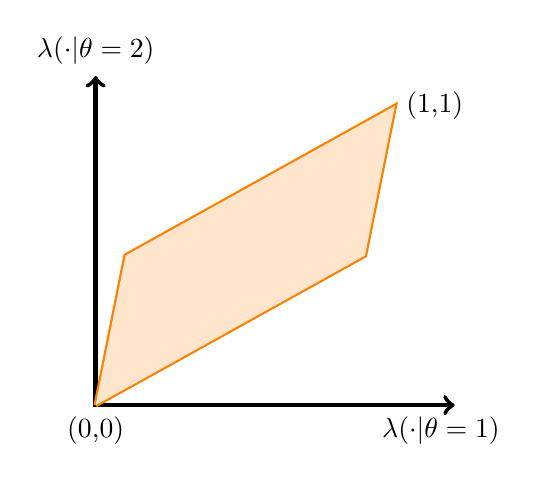
\begin{tikzpicture}[domain=0:3, scale=3.8, ultra thick]    


	\draw[<->] (0,1.1) node[above]{$\lambda(\cdot|\theta=2)$} -- (0,0)node[below]{(0,0)}-- (1.2,0) node[below,xshift=-5]{$\lambda(\cdot|\theta=1)$};
	  
	\draw[orange] (0,0)--(0.1,0.5)--(1,1)--(0.9,0.5)--(0,0);
	\fill[orange!20] (0,0)--(0.1,0.5)--(1,1)--(0.9,0.5)--(0,0);
	\draw (1,1)node[right]{(1,1)};
%	\draw[orange] (1,0.9)node[right]{$\Lambda_{P_1}$};
	
	\end{tikzpicture}   
}
\hspace{0.2in}
\subfigure[$\Lambda_{\overline{P}}$ as the convex hull of $\Lambda_{P_1}\cup \Lambda_{P_2}$]
{
	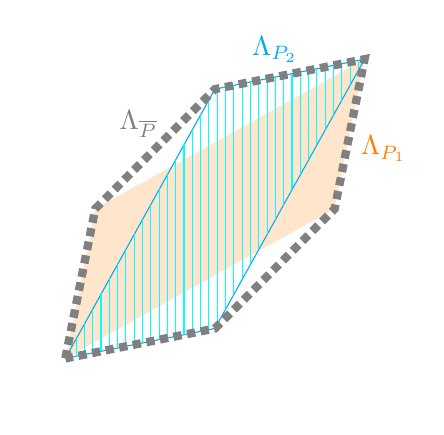
\begin{tikzpicture}[domain=0:3, scale=3.8, ultra thick]    
%	\draw[<->] (0,1.1) node[left]{} -- (0,0)-- (1.2,0) node[below,xshift=-5]{};
	  
%	\draw[orange] (0,0)--(0.1,0.5)--(1,1)--(0.9,0.5)--(0,0);
	\fill[orange!20] (0,0)node[below,white]{(0,0)}--(0.1,0.5)--(1,1)--(0.9,0.5)--(0,0);
	\draw[orange] (0.95,0.7)node[right]{$\Lambda_{P_1}$};
	
	\draw[cyan,thin] (0,0)--(0.5,0.9)--(1,1)--(0.5,0.1)--(0,0);
	\fill[pattern=vertical lines, pattern color=cyan] (0,0)--(0.5,0.9)--(1,1)--(0.5,0.1)--(0,0);
	\draw[cyan] (0.7,0.95)node[above]{$\Lambda_{P_2}$};
	
	\draw[gray,dotted,line width=3] (0,0)--(0.1,0.5)--(0.5,0.9)--(1,1)--(0.9,0.5)--(0.5,0.1)--(0,0);
	\draw[gray] (0.3,0.7)node[above,xshift=-6]{$\Lambda_{\overline{P}}$};
	
%	\draw[red] (0,0.6)--(0.5,0.9)--(1,1.2);
%	\draw[red] (0.3,0.9)node[above]{$u\cdot \lambda=c$};
%    \draw[red,->] (0.5,0.9)--(0.41,1.05)node[right,xshift=2]{$u$};
	
	\end{tikzpicture}  
}
	
	\caption{}
	\label{zonotope}
\end{figure}
\section{Nature's Problem}

Most of our focus will be on the robustly optimal strategies for the agent, but it will be helpful to first understand Nature's problem, of choosing the worst possible correlation structure. 

First note that since the objective function is linear in both $\sigma$ and $P$, and the choice sets of $\sigma$ and $P$ are both convex and compact, the minimax theorem implies that
	\[
	V(P_1, \ldots , P_m)= \min_{P \in \mathcal{P}(P_1, \ldots , P_m)} \max_{\sigma\in\Sigma}  \sum_{\theta\in\Theta}\sum_{(y_1, \ldots , y_m) \in \mathbf{Y}} P(y_1, \ldots , y_m|\theta)  u(\theta,\sigma(y_1, \ldots , y_m)).
	\]
That is, the value of the agent's maxmin problem equals the value of a minmax problem where Nature chooses an experiment in the set $\mathcal{P}(P_1, \ldots , P_m)$ to minimize a Bayesian agent's value in the decision problem. 

An immediate observation is that if there exists a Blackwell least informative element in the set $\mathcal{P}(P_1, \ldots , P_m)$, it would solve Nature's problem---any other information structure would yield a higher value for the agent. Notice that every experiment in $\mathcal{P}(P_1, \ldots , P_m)$ must be more informative than every $P_j$, since the projection into the $j$th coordinate defines a garbling. By Lemma \ref{lem:blackwellsup}, there is a \emph{Blackwell supremum}---the least informative experiment that Blackwell dominates every $P_j$. The only question that remains is whether this Blackwell supremum can be expressed as a joint distribution with marginals $P_1,\ldots, P_m$. This is proved in the following lemma.

\begin{lem}\label{lem:supjoint}
For any collection of experiments $\{P_j\}_{j=1}^m$, there exists a Blackwell supremum $\overline{P}(P_1,\ldots,P_m)\in \mathcal{P}(P_1, \ldots , P_m)$ so that for any $P\in \mathcal{P}(P_1, \ldots , P_m)$, $V(\overline{P}(P_1,\ldots,P_m))\leq V(P)$.

%$\overline{P}(P_1,\ldots,P_m)\in \mathcal{P}(P_1, \ldots , P_m)$.
\end{lem}
\begin{proof}
See Appendix~\ref{proof:blackwellsup}.
\end{proof}

Immediately from the lemma, we have the following proposition.
\begin{prop}\label{value}
    $$V(P_1,...,P_m)=V(\overline{P}(P_1,...,P_m))$$
    where $\overline{P}(P_1,...,P_m)$ is a Blackwell supremum of experiments $\{P_1,...,P_m\}$.
\end{prop}

Thus, the agent's value from using a robust strategy is the same as the value she would obtain if she faced a single experiment---the Blackwell supremum of all marginal experiments. Moreover, the Blackwell supremum depends only on the marginal experiments, and not on the particular decision problem.


\section{Binary Action Decision Problems}\label{sec:binarybinary}




While \autoref{value} provides a useful characterization of the agent's value, it still does not answer our main question: what are the robust strategies? This is because a strategy may be a best response to the Blackwell supremum $\bar{P}(P_1, \ldots , P_m)$, without being a robustly optimal strategy. In particular, the Blackwell supremum typically specifies a probability of zero for many signal realizations, so that any action is a best response to those signal realizations. But if we fix a strategy that chooses a particularly bad action after such a signal realization, it might be a best response for Nature to make it occur with positive probability. So we now turn to the question of finding the optimal robust strategies.  

 

For any decision problem, one simple strategy that can always be used is to choose exactly one experiment $Q \in \{P_1, \ldots ,P_m\}$ and play the optimal strategy that uses that information alone, ignoring the signal realizations of all other experiments. By choosing $Q$ optimally, the agent achieves an ex-ante expected payoff of $\max_{j = 1, \ldots , n} V(P_j)$, regardless of the particular actual joint experiment $P \in \mathcal{P}(P_1, \ldots , P_m)$.  \autoref{binary} shows that if the decision problem has binary action, this is indeed a robustly optimal strategy.

\begin{thm}\label{binary}
    If $|A| = 2$, then 
    \[
    V(P_1, \ldots , P_m) = V(\overline{P}(P_1, \ldots , P_m)) =  \max_{j = 1, \ldots , m}V(P_j).
    \]
\end{thm}


\begin{proof}
By \autoref{value}, it suffices to show that $V(\overline{P}(P_1,...,P_m))=\max_{j=1,...,m}V(P_j)$.
By \autoref{lem:blackwellsupfeasible}, an experiment $\overline{P}$ is the Blackwell supremum of $P_1,\ldots,P_m$ if and only if
\begin{equation}\label{convex_hull}
\Lambda_{\overline{P}} =co\left(\Lambda_{P_1}\cup \cdots \cup \Lambda_{P_m}\right)    
\end{equation}
Now, the maximum utility achievable given Blackwell experiment  $\overline{P}(P_1, \ldots , P_m)$ is
$V(\overline{P})=\max_{\lambda\in \Lambda_{\overline{P}}}\sum_{a,\theta} u(\theta,a)\lambda(a|\theta)$.
Since the maximand is linear in $\lambda$, the maximum is achieved at an extreme point of $\Lambda_{\overline{P}}$. By (\ref{convex_hull}), an extreme point of $\Lambda_{\overline{P}}$ must belong to some $\Lambda_{P_j}$. Hence, we have
$$V(\overline{P})=\max_{\lambda\in \Lambda_{P_j}}\sum_{a,\theta} u(\theta,a)\lambda(a|\theta)=\max_{j=1,...,m}V(P_j).$$
\end{proof}

\begin{figure}
\centering
	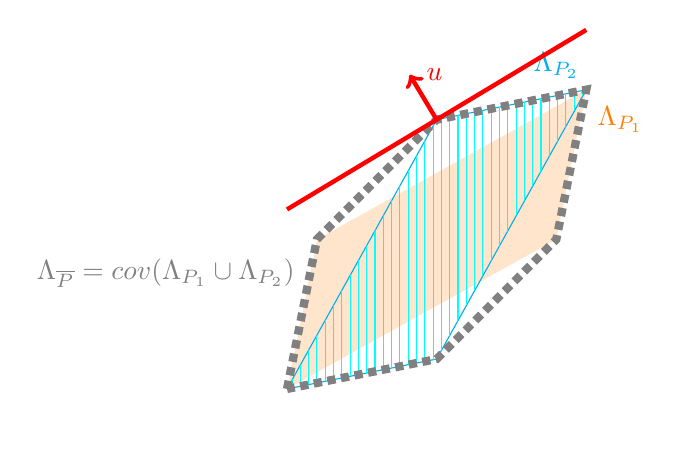
\begin{tikzpicture}[domain=0:3, scale=3.8, ultra thick]    


	\fill[orange!20] (0,0)node[below,white]{(0,0)}--(0.1,0.5)--(1,1)--(0.9,0.5)--(0,0);
	\draw[orange] (1,0.9)node[right]{$\Lambda_{P_1}$};
	
	\draw[cyan,thin] (0,0)--(0.5,0.9)--(1,1)--(0.5,0.1)--(0,0);
	\fill[pattern=vertical lines, pattern color=cyan] (0,0)--(0.5,0.9)--(1,1)--(0.5,0.1)--(0,0);
	\draw[cyan] (0.9,1)node[above]{$\Lambda_{P_2}$};
	
	\draw[gray,dotted,line width=3] (0,0)--(0.1,0.5)--(0.5,0.9)--(1,1)--(0.9,0.5)--(0.5,0.1)--(0,0);
	\draw[gray] (-0.35,0.3)node[above,xshift=-6]{$\Lambda_{\overline{P}}=cov(\Lambda_{P_1}\cup \Lambda_{P_2})$};
	
	\draw[red] (0,0.6)--(0.5,0.9)--(1,1.2);

    \draw[red,->] (0.5,0.9)--(0.41,1.05)node[right,xshift=2]{$u$};
	
	\end{tikzpicture}  
	\caption{The maximum is achieved at an extreme point}
	\label{extreme}
\end{figure}

The idea of \autoref{binary} can be visualized in \autoref{extreme} for two marginal experiments. Each marginal Blackwell experiment $P_1,P_2$ can be represented by $\Lambda_{P_1},\Lambda_{P_2}$, the set of feasible state-action distribution generated by the experiment. The corresponding $\Lambda_{\overline{P}}$ for Blackwell supremum $\overline{P}$ is the convex hull of $\Lambda_{P_1}\cup \Lambda_{P_2}$. Since the utility function is linear with respect to $\lambda \in \Lambda_{\overline{P}}$, the maximum is achieved at an extreme point, which belongs to either $\Lambda_{P_1}$ or $\Lambda_{P_2}$, and thus can be achieved by using a single marginal experiment.


\section{General Decision Problems}\label{sec:binarygen}

\autoref{binary} allows us to solve any binary action decision problem in a fairly simple way: finding the best marginal information source and best responding to it. For decision problem with more actions, a robustly optimal strategy may need to use multiple information sources. 

To understand how optimal robust strategies work in general, we start our discussion in \autoref{sec:example} and \autoref{sec:composition} with a simple class of decision problems: those that can be written as a composition of multiple binary action problems. For these problems, we show that the optimal strategy can be obtained by simply ``adding up'' the optimal strategies for the isolated binary action problems. Finally, in \autoref{sec:decompose} and \autoref{sec:canonical}, we show that this simple class of decision problems is exhaustive---\textbf{any} finite action decision problem can be decomposed into binary action decision problems.




\subsection{An Example}\label{sec:example}

We start with an example which showcases how an agent can benefit from using information from multiple sources when she faces a more complex problem.

\begin{ex}\label{ex-portfolio}


An investor can invest in two assets whose outputs depend on an unknown binary state $\theta\in\{1,2\}$. Outputs from each asset are given by:


\vspace{0.1in}
\hspace{0.5in}\begin{tabular}{  |c | c |c|}
           
           \multicolumn{3}{c}{Asset 1}      \\\hline
           &  Invest & Not Invest\\ \hline
          $\theta=1$ & $2$ & $0$\\ \hline
          $\theta=2$ & $-1$ & $0$\\ \hline
\end{tabular}
\hfill
\begin{tabular}{  |c | c |c|}
           \multicolumn{3}{c}{Asset 2}      \\\hline
           &  Invest & Not Invest\\ \hline
          $\theta=1$ & $-1$ & $0$\\ \hline
          $\theta=2$ & $2$ & $0$\\ \hline
\end{tabular}
\hspace{0.5in}
\vspace{0.2in}

\noindent The investor's payoff is the sum of outputs from both assets. This can be written as a decision problem with $A=\{I,NI\}\times \{I,NI\}$ and $u(\theta,a)=u_1(\theta,a_1)+u_2(\theta,a_2)$ where $a_1,a_2\in\{I,NI\}$ and $u_1,u_2$ are the outputs function given in the table above.\footnote{Recall that $u(\theta,a)=\nu(\theta)\rho(\theta,a)$, so the payoffs here have been weighted by the prior.}

Suppose the investor has access to two experiments $P_1$, $P_2$: 


\vspace{0.1in}
\hspace{0.5in}\begin{tabular}{  |c | c |c|}
           
           \multicolumn{3}{c}{$P_1$}      \\\hline
           &  $y_1=1$ & $y_1=0$\\ \hline
          $\theta=1$ & $0.9$ & $0.1$\\ \hline
          $\theta=2$ & $0.5$ & $0.5$\\ \hline
\end{tabular}
\hfill
\begin{tabular}{  |c | c |c|}
          \multicolumn{3}{c}{$P_2$}      \\ \hline
        &  $y_2=1$ & $y_2=0$\\ \hline
          $\theta=1$ & $0.5$ & $0.5$\\ \hline
          $\theta=2$ & $0.9$ & $0.1$\\ \hline
\end{tabular}
\hspace{0.5in}
\vspace{0.2in}



By paying attention to one experiment, for example $P_1$, the optimal strategy is to invest in both assets if $y_1=1$ and only asset $2$ if $y_1=0$. The expected payoff from this strategy is thus $0.9\cdot 1+0.1\cdot (-1)+0.5\cdot 1+0.5\cdot 2=2.3$.

Now suppose the investor makes the investment decision of asset 1 based on experiment $P_1$, and asset 2 based on experiment $P_2$. Then for asset $i=1,2$, the optimal strategy is to invest iff $y_{i}=1$. ``Adding up'' these two strategies yield:

\begin{center}
     \begin{tabular}{  |c | c |c|}
           \hline
        &  $y_2=1$ & $y_2=0$\\ \hline
          $y_1=1$  & Invest in both & Invest in asset 1\\ \hline
            $y_1=0$  & Invest in asset 2 & No investment\\ \hline
    \end{tabular}
\end{center}

This strategy guarantees an expected output of $0.9\cdot 2+0.1\cdot 0+0.5\cdot (-1)+0.5\cdot 0=1.3$ from each asset regardless of the correlations, which gives a total output of $2.6>2.3$. So the agent strictly benefits from utilizing information from both information sources.
\end{ex}



The strategy constructed in \autoref{ex-portfolio} is in fact a robustly optimal strategy. There are two special structures of this example: 1. The action space is a product space of binary action spaces; 2. The payoff function can be written in an additively separable form of binary action problems. These two features enable us to find a robustly optimal strategy in a fairly simple way: find the robustly optimal strategy for each binary action problem via \autoref{binary}, and then ``add them up''. We will generalize and formalize this idea in the next section.




\subsection{Composition of Decision Problems}\label{sec:composition}

Recall that we define a decision problem as $\Gamma\equiv (\Theta,\nu,A,\rho)$, which can simply be summarized by $(A,u)$ where $u(\theta,a)=\nu(\theta)\rho(\theta,a)$. Since in this section we are going to alter the decision problems along the analyses, we use $V(P_1,...,P_m;(A,u))$ to denote the agent's value in decision problem $(A,u)$.



\begin{defn}
Given a finite collection of decision problems $(A_1,u_1),...,(A_n,u_n)$, their composition, denoted by $\bigoplus_{\ell=1}^k (A_\ell,u_\ell)$, is a decision problem with action space $A=(A_1\times\ldots\times A_k)$ and $u(\theta,\mathbf{a})=\sum_{\ell=1}^k u_\ell(\theta,a_\ell)$.
\end{defn}

Thus, the composition of decision problems is a single decision problem that has a specific additively separable structure. Notice that the decision problem in \autoref{ex-portfolio} is a composition of two decision problems $A_1=\{I_1,N_1\}$, $A_2=\{I_2,N_2\}$ and $u_1(\cdot,I_1)=(2,-1)$, $u_1(\cdot,N_1)=(0,0)$, $u_2(\cdot,I_2)=(-1,2)$, $u_2(\cdot,N_2)=(0,0)$.






Consider a finite collection of \textbf{binary} action problems, $(A_1, u_1), \ldots , (A_k, u_k)$, and consider the composition of these problems $(\bar{A}, \bar{U}) := \bigoplus_{\ell = 1}^k (A_\ell, u_\ell)$.  In this decision problem, a simple, robust strategy that an agent can always use is to choose exactly one experiment $Q_\ell \in \{P_1, \ldots , P_m\}$ for every binary problem $\ell$ and play the optimal strategy that uses that information alone, ignoring the signal realizations of all other experiments.  Furthermore, by choosing this $Q_\ell$ optimally for each $\ell$, regardless of the actual joint experiment $P \in \mathcal{P}(P_1, \ldots , P_m)$,  the agent can achieve a total ex-ante utility of $\sum_{\ell = 1}^{k} \max_{j = 1, \ldots , m}V(P_j, (A_\ell, u_\ell))$,  which is typically strictly greater than $\max_{j  = 1, \ldots , m} V(P_j, (\bar{A}, \bar{U}))$.
The following lemma shows that this is indeed the best that the agent can do in $(\bar{A}, \bar{U})$.

\begin{lem}\label{lem:decomposed}
    Let $(A_1, u_1), \ldots , (A_k, u_k)$ be a finite collection of \textbf{binary} action problems.  Then
    \[
    V\left(P_1, \ldots , P_m; \bigoplus_{\ell = 1}^{k} (A_\ell, u_\ell)\right) = \sum_{\ell = 1}^{k} \max_{j = 1, \ldots, m} V(P_j; (A_\ell, u_\ell)).
    \]
    
Moreover, let $\sigma_\ell:\mathbf{Y}\rightarrow \Delta A_\ell$ be a robustly optimal strategy for decision problem $(A_\ell,u_\ell)$. Then $\sigma:\mathbf{Y}\rightarrow \Delta (A_1\times ...\times A_k)$ defined by
\begin{equation}\label{eq:assemble}
\sigma(y_1,...,y_m)=\bigg(\sigma_\ell(y_1,...,y_m)\bigg)_{\ell=1}^k\quad\text{ for all }y_1,...,y_m
\end{equation}
is a robustly optimal strategy for decision problem $\bigoplus_{\ell = 1}^{k} (A_\ell, u_\ell)$.
\end{lem}


\begin{proof}
Using \autoref{value}, 
$V\left(P_1, \ldots , P_m; \bigoplus_{\ell = 1}^{k} (A_\ell, u_\ell)\right) = V\left(\overline{P}(P_1, \ldots , P_m); \bigoplus_{\ell = 1}^{k} (A_\ell, u_\ell) \right)$.
By \autoref{binary}, we then have:
\[
V\left(\overline{P}(P_1, \ldots , P_m); \bigoplus_{\ell = 1}^{k} (A_\ell, u_\ell) \right) = \sum_{\ell = 1}^{k} V(\overline{P}(P_1, \ldots , P_m); (A_\ell, u_\ell)) = \sum_{\ell = 1}^{k} \max_{j = 1, \ldots , m}V(P_j, (A_\ell,u_\ell)).
\]
To see the second statement, for any $P\in\mathcal{P}(P_1,...,P_m)$, the agent's payoff from strategy $\sigma$ is
\begin{align*}
    \sum_{\theta\in\Theta}\sum_{y_1,...,y_m} P(y_1,...,y_m|\theta) \sum_{\ell=1}^k u_\ell(\theta,\sigma_\ell(y_1,...,y_m))&= \sum_{\ell=1}^k\sum_{\theta\in\Theta}\sum_{y_1,...,y_m} P(y_1,...,y_m|\theta)  u_\ell(\theta,\sigma_\ell(y_1,...,y_m))\\
    &\geq \sum_{\ell=1}^k V(P_1,...,P_m;(A_\ell,u_\ell))\\
%    &=\sum_{\ell = 1}^{k} \max_{j = 1, \ldots, m} V(P_j, (A_\ell, u_\ell))\\
    &=  V\left(P_1, \ldots , P_m; \bigoplus_{\ell = 1}^{k} (A_\ell, u_\ell)\right)
\end{align*}
%where the inequality holds from the definition of $\sigma_\ell$, the second equality holds from \autoref{binary}, and the last equality is \autoref{lem:decomposed}. 
Since $\sigma$ guarantees the maxmin value regardless of $P$, it is a robustly optimal strategy.
\end{proof}

\autoref{lem:decomposed} provides a simple solution to any problem that can be expressed as a composition of binary action problem: For each binary action problem, one can derive a robustly optimal strategy by paying attention to the best marginal experiment and best responding to it. Then assembling these strategies as in \eqref{eq:assemble} yields a robustly optimal strategy for the composite problem.

\subsection{Decomposition of decision problems}\label{sec:decompose}

In the previous section, we saw how a problem that is a composition of binary action problems can be solved by combining the solutions of each binary action problem. It is natural to ask then what problems can be decomposed into binary action problems. As we will see in the next section, it turns out that such a decomposition is possible for any decision problem. Before we get to that, we must define precisely what it means to decompose a decision problem and for that we need a notion of equivalence between decision problems. 


For each decision problem $(A,u)$, define the associated polyhedron containing all payoff vectors that are either achievable or weakly dominated by some mixed action:\footnote{Here and in what follows, whenever $+$ and $-$ are used in the operations of sets, they denote the Minkowski sum and difference.}
\[\po(A,u)=co\{u(\cdot,a):a\in A\}-\mathbb{R}_+^{2}.\]
An example of $\po(A,u)$ is depicted in \autoref{figure-actionorder}.

\begin{figure}[htp]
	\centering

	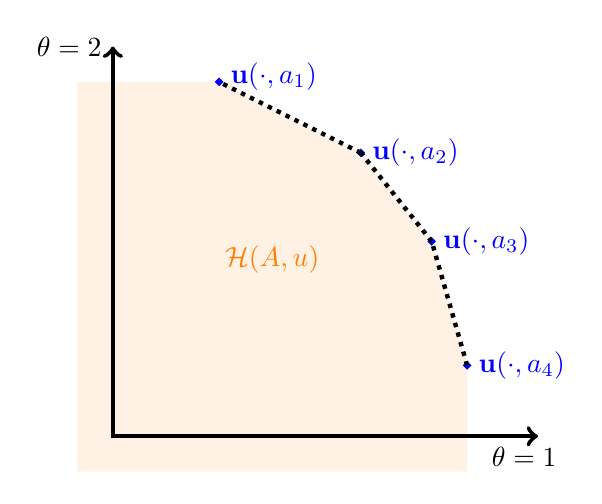
\begin{tikzpicture}[domain=0:3, scale=4.5, ultra thick]    
	
%   \fill[orange!15] (0,0)--(1,0)--(1,0.3)--(0.8,0.7)--(0.4,1.1)--(0,1.1)--(0,0);
    \fill[orange!10] (-0.1,-0.1)--(1,-0.1)--(1,0.2)--(0.9,0.55)--(0.7,0.8)--(0.3,1)--(-0.1,1)--(-0.1,-0.1);
    
	\draw[<->] (0,1.1) node[left]{$\theta=2$} -- (0,0)-- (1.2,0) node[below,xshift=-5]{$\theta=1$};
	
   
    
    \filldraw[blue] (1,0.2)circle (0.1pt)node[right]{$\bu(\cdot,a_4)$};
    \filldraw[blue] (0.9,0.55)circle (0.1pt)node[right]{$\bu(\cdot,a_3)$};
    \filldraw[blue] (0.7,0.8)circle (0.1pt)node[right]{$\bu(\cdot,a_2)$};
    \filldraw[blue] (0.3,1)circle (0.1pt)node[right,yshift=2]{$\bu(\cdot,a_1)$};
    
	\draw[dotted] (1,0.2)--(0.9,0.55);
	\draw[dotted] (0.9,0.55)--(0.7,0.8);
	\draw[dotted] (0.7,0.8)--(0.3,1);

    \draw[orange] (0.45,0.5)node{$\po(A,u)$};
	
	\end{tikzpicture}   
	\caption{The shaded area represents $\po(A,u)$}
   \label{figure-actionorder}
\end{figure}

Whenever $\po(A',u')= \po(A,u)$, the two decision problems $\po(A',u')$ and $\po(A,u)$ give the same value under any information environment, so we call them \emph{equivalent}.

\begin{defn}
A decision problem $(A,u)$ is equivalent to another decision problem $(A',u')$ if 
\[\po(A',u')= \po(A,u).\]
\end{defn}


Now we can define decomposition, the inverse operation of composition:
\begin{defn}
A decision problem $(A,u)$ admits a decomposition $\{(A_\ell,u_\ell)\}_{\ell=1}^k$ if $(A,U)$ is equivalent to $\bigoplus_{\ell=1}^k (A_\ell,u_\ell)$.
\end{defn}


\begin{ex}\label{ex-decomposition}
Consider two decision problems $A_1=\{I_1,N_1\}$, $u_1(I_1)=(2,-1)$, $u_1(N_1)=(0,0)$ and $A_2=\{I_2,N_2\}$, $u_2(I_2)=(-1,2)$, $u_2(N_2)=(0,0)$. The associated polyhedra are the blue/red shaded areas in \autoref{figure-ex-composition}(a). Their composition $(A_1,u_1)\bigoplus (A_2,u_2)$ consists of four actions, which are depicted in \autoref{figure-ex-composition}(b).


Now we consider a three-action decision problem $A=\{a_1,a_2,a_3\}$ with $u(a_1)=(-1,2), u(a_2)=(1,1)$, and $u(a_3)=(2,-1)$. Notice that $\po(A,u)=\po((A_1,u_1)\bigoplus (A_2,u_2))$ as the shaded area in \autoref{figure-ex-composition}(b), so $(A,u)$ is equivalent to $(A_1,u_1)\bigoplus (A_2,u_2)$. Therefore, $(A_1,u_1),(A_2,u_2)$ is a decomposition of $(A,u)$.
\end{ex}


\begin{figure}[htp]  
	\centering  
	\small
	%figure(a)
	\subfigure[Polyhedra induced by $(A_1,u_1)$ and $(A_2,u_2)$]  
	{  
		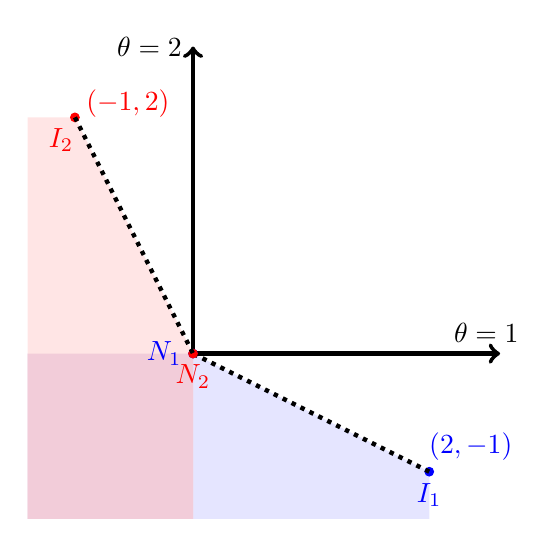
\begin{tikzpicture}[domain=0:3, scale=3, ultra thick]
			\fill[blue!10] (-0.2,-0.2)--(1.5,-0.2)--(1.5,0)--(0.5,0.5)--(-0.2,0.5)--(-0.2,-0.2);
			\fill[red!10] (-0.2,-0.2)--(0.5,-0.2)--(0.5,0.5)--(0,1.5)--(-0.2,1.5)--(-0.2,-0.2);
			\fill[purple!20]  (-0.2,-0.2)--(0.5,-0.2)--(0.5,0.5)--(-0.2,0.5)--(-0.2,-0.2);
			
			\draw[<->] (0.5,1.8) node[left]{$\theta=2$} -- (0.5,0.5)-- (1.8,0.5) node[above,xshift=-5]{$\theta=1$};
			
			\filldraw[blue] (1.5,0)circle (0.3pt)node[below]{$I_1$};
			\filldraw[blue] (0.5,0.5)circle (0.3pt)node[left]{$N_1$};
			
			\draw[dotted] (1.5,0)--(0.5,0.5);
			
			%   \draw[orange] (0.15,0.15)node{$\po(A,u)$};
			
			\filldraw[red] (0,1.5)circle (0.3pt)node[below,xshift=-5]{$I_2$};
			\filldraw[red] (0.5,0.5)circle (0.3pt)node[below]{$N_2$};  
			\draw[dotted] (0,1.5)--(0.5,0.5);
			
				\draw[blue] (1.5,0)node[above,xshift=15]{$(2,-1)$};
				\draw[red]  (0,1.5)node[right,yshift=5]{$(-1,2)$} ;
			
		\end{tikzpicture}  
	}  
	\hspace{0.01in}
	%figure(b)
	\subfigure[Polyhedron induced by $(A_1,u_1)\bigoplus (A_2,u_2)$]  
	{  
		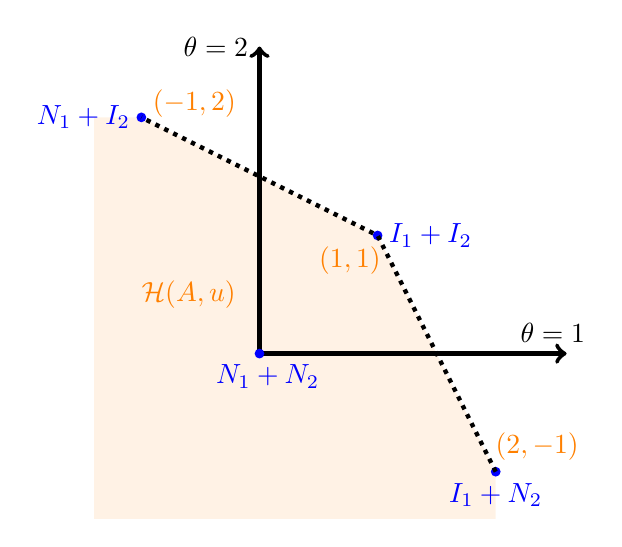
\begin{tikzpicture}[domain=0:3, scale=3, ultra thick]
			\fill[orange!10] (-0.2,-0.2)--(1.5,-0.2)--(1.5,0)--(1,1)--(0,1.5)--(-0.2,1.5)--(-0.2,-0.2);
			
		\draw[<->] (0.5,1.8) node[left]{$\theta=2$} -- (0.5,0.5)-- (1.8,0.5) node[above,xshift=-5]{$\theta=1$};
			
			
			
			\filldraw[blue] (1.5,0)circle (0.3pt)node[below]{$I_1+N_2$};
			\filldraw[blue] (1,1)circle (0.3pt)node[right]{$I_1+I_2$};
			\filldraw[blue] (0,1.5)circle (0.3pt)node[left]{$N_1+I_2$};
			\filldraw[blue] (0.5,0.5)circle (0.3pt)node[below,xshift=3]{$N_1+N_2$};
			
			\draw[dotted] (1.5,0)--(1,1)--(0,1.5);
			
			\draw[orange] (1.5,0)node[above,xshift=15]{$(2,-1)$} (1,1)node[below,xshift=-10]{$(1,1)$} (0,1.5)node[right,yshift=5]{$(-1,2)$} ;
			\draw[orange] (0.2,0.75)node{$\po(A,u)$};
			
			
		\end{tikzpicture}  
		
	}

	\caption{}
	\label{figure-ex-composition}
\end{figure}




The analyses in the previous section give some hint on how to find robustly optimal strategies for general decision problems. If a given decision problem $(A, u)$ admits a decomposition $(A_1, u_1), \ldots , (A_k, u_k)$ where each $(A_\ell,u_\ell)$ is a \textbf{binary} action problem, then it is immediately clear by \autoref{lem:decomposed} and $\po\left( A, u\right) = \po\left(\bigoplus_{\ell =1}^{k}(A_\ell, u_\ell) \right)$ that
\begin{align}
V(P_1, \ldots P_m; (A, u)) = V\left(P_1, \ldots , P_m; \bigoplus_{\ell = 1}^{k} (A_\ell, u_\ell)\right) = \sum_{\ell = 1}^{k} \max_{j = 1, \ldots , m}V(P_j; (A_\ell, u_\ell)). \label{eqn:canonical}
\end{align}
Moreover, the robustly optimal strategy for $\bigoplus_{\ell = 1}^{k} (A_\ell, u_\ell)$, defined in \eqref{eq:assemble}, allows us to characterize robustly optimal strategies for $(A,u)$ as by the following lemma.

\begin{lem}\label{lem:dominate}
Suppose $(A,u)$ is equivalent to $\bigoplus_{\ell = 1}^{k} (A_\ell, u_\ell)$, and $\sigma:\mathbf{Y}\rightarrow \Delta(A_1\times\ldots\times A_k)$ is a robustly optimal strategy for $\bigoplus_{\ell = 1}^{k} (A_\ell, u_\ell)$, then there exists $\sigma^*:\mathbf{Y}\rightarrow \Delta A$ such that
\[u(\sigma^*(\mathbf{y}))\geq \sum_{\ell=1}^k u_\ell(\sigma_\ell(\mathbf{y})),\quad\text{ for all }\mathbf{y} \in \mathbf{Y}.\]
Moreover, any such $\sigma^*$ is a robustly optimal strategy for $(A,u)$.
\end{lem}
\begin{proof}
For each $\mathbf{y}$, $\sum_{\ell=1}^k u_\ell(\sigma_\ell(\mathbf{y}))\in \po\bigg(\bigoplus_{\ell = 1}^{k} (A_\ell, u_\ell)\bigg)=\po(A,u)$. So there exists $\sigma^*(\mathbf{y})$ such that $u(\sigma^*(\mathbf{y}))\geq \sum_{\ell=1}^k u_\ell(\sigma_\ell(\mathbf{y}))$. Moreover, since $\sigma^*$ guarantees a higher value in $(A,u)$ than $\sigma$ in $\bigoplus_{\ell = 1}^{k} (A_\ell, u_\ell)$, and $V(P_1, \ldots P_m; (A, u)) = V\left(P_1, \ldots , P_m; \bigoplus_{\ell = 1}^{k} (A_\ell, u_\ell)\right)$, $\sigma^*$ is a robustly optimal strategy for $(A,u)$.
\end{proof}



If a decision problem $(A, u)$ admits a decomposition into binary action problems, \autoref{lem:decomposed} and \autoref{lem:dominate} characterize a set of robustly optimal strategies. However, it is not immediately clear what kind of decision problem admits a decomposition into binary action problems. Interestingly, we show by direct construction that, \textbf{any}  decision problem admits a decomposition into binary action problems.



\subsection{Canonical Decomposition}\label{sec:canonical}

We are now ready to show that any decision problem can be decomposed into binary-action problems. Given an arbitrary decision problem $(A,u)$, we start with some normalization to simplify exposition. First we remove all weakly*-dominated actions,\footnote{An action $a\in A$ is weakly*-dominated if there exists $\alpha\in \Delta A$ such that $u(a)\leq u(\alpha)$. If there are duplicated actions, we remove all but keep one copy.} so that actions can be ordered as
\begin{align*}
 u(\theta_1,a_1) < u(\theta_1,a_2) < \cdots < u(\theta_1,a_n),\\
 u(\theta_2,a_1) > u(\theta_2,a_2) > \cdots > u(\theta_2,a_n).
\end{align*}
Moreover, by adding a constant vector, we can normalize $u(\cdot,a_1)=(0,0)$. 



\begin{defn}
Given a decision problem $(A, u)$, the \textbf{canonical decomposition} of $(A, u)$ is the following collection of $n - 1$ binary action problems $(A_1^*, u_1^*), \ldots , (A_{n - 1}^*, u_{n-1}^*)$:
\[
A_{\ell}^* := \left\{0, 1 \right\}, u_\ell^*(\cdot,0) = (0,0), u_\ell^*(\cdot,1) = u(\cdot,a_{\ell + 1}) - u(\cdot,a_{\ell}).
\]
\end{defn}



\begin{figure}[t]
	\centering
\subfigure[Canonical decomposition]{
		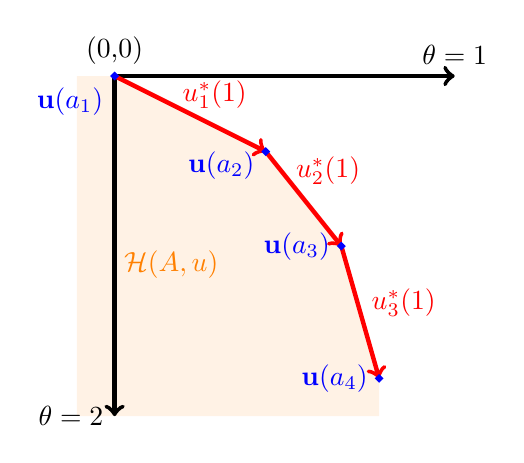
\begin{tikzpicture}[domain=0:3, scale=4.8, ultra thick]    
	
    \fill[orange!10] (0.2,0.1)--(1,0.1)--(1,0.2)--(0.9,0.55)--(0.7,0.8)--(0.3,1)--(0.2,1)--(0.2,0.1);
    
	\draw[<->] (0.3,0.1)node[left]{$\theta=2$}--(0.3,1)node[above]{(0,0)}--(1.2,1)node[above]{$\theta=1$};
   
   
    \draw[red,<-] (0.7,0.8)--(0.3,1) ;
 	\draw[red] (0.45,0.95)node[right]{$u^*_1(1)$};
 	
 	\draw[red,<-] (0.9,0.55)--(0.7,0.8);
 	\draw[red] (0.75,0.75)node[right]{$u^*_2(1)$};
    
	\draw[red,<-] (1,0.2)--(0.9,0.55);
 	\draw[red] (0.95,0.4)node[right]{$u^*_3(1)$};
    
    \filldraw[blue] (1,0.2)circle (0.1pt)node[left]{$\bu(a_4)$};
    \filldraw[blue] (0.9,0.55)circle (0.1pt)node[left]{$\bu(a_3)$};
    \filldraw[blue] (0.7,0.8)circle (0.1pt)node[left,yshift=-5]{$\bu(a_2)$};
    \filldraw[blue] (0.3,1)circle (0.1pt)node[below left]{$\bu(a_1)$};

 


    \draw[orange] (0.45,0.5)node{$\po(A,u)$};
	
	\end{tikzpicture}   
}
\hspace{0.1in}
\subfigure[Nonconsecutive sum lies in the interior]{
	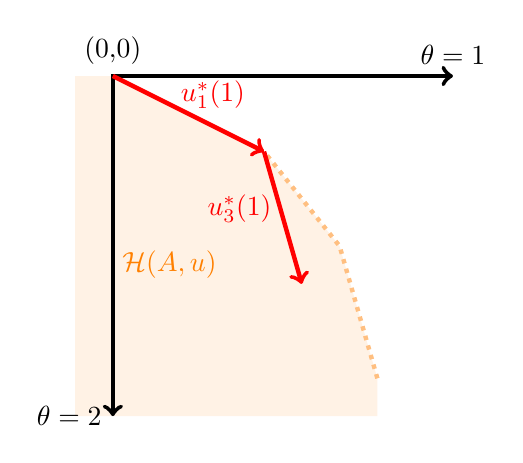
\begin{tikzpicture}[domain=0:3, scale=4.8, ultra thick]    
	
%   \fill[orange!15] (0,0)--(1,0)--(1,0.3)--(0.8,0.7)--(0.4,1.1)--(0,1.1)--(0,0);
    \fill[orange!10] (0.2,0.1)--(1,0.1)--(1,0.2)--(0.9,0.55)--(0.7,0.8)--(0.3,1)--(0.2,1)--(0.2,0.1);
    
%	\draw[<->] (0,1.1) node[left]{$\theta=2$} -- (0,0)-- (1.2,0) node[below,xshift=-5]{$\theta=1$};
	\draw[<->] (0.3,0.1)node[left]{$\theta=2$}--(0.3,1)node[above]{(0,0)}--(1.2,1)node[above]{$\theta=1$};
   
   
    \draw[dotted,orange!50] (1,0.2)--(0.9,0.55)--(0.7,0.8);
   
    \draw[red,<-] (0.7,0.8)--(0.3,1) ;
 	\draw[red] (0.45,0.95)node[right]{$u^*_1(1)$};
 	
 %	\draw[red,<-] (0.9,0.55)--(0.7,0.8);
 %	\draw[red] (0.75,0.75)node[right]{$u^*_2(1)$};
    
	\draw[red,<-] (0.8,0.45)--(0.7,0.8);
 	\draw[red] (0.75,0.65)node[left]{$u^*_3(1)$};
    
 %   \filldraw[blue] (1,0.2)circle (0.1pt)node[left]{$\bu(a_4)$};
%    \filldraw[blue] (0.9,0.55)circle (0.1pt)node[left]{$\bu(a_3)$};
%    \filldraw[blue] (0.7,0.8)circle (0.1pt)node[left,yshift=-5]{$\bu(a_2)$};
 %   \filldraw[blue] (0.3,1)circle (0.1pt)node[left]{$\bu(a_1)$};
    

 


    \draw[orange] (0.45,0.5)node{$\po(A,u)$};
	
	\end{tikzpicture}   
}
	
	\caption{}
	\label{figure:canonical}
\end{figure}




The canonical decomposition can be visualized in \autoref{figure:canonical} for an example with four actions. To see that a canonical decomposition is a decomposition, first notice that for any $i=1,...,n$, $u(a_i)=\sum_{\ell=1}^{i-1}u^*_{\ell}(1)+\sum_{\ell=i}^{n-1}u^*_{\ell}(0)$, so $\po(A,u)\subset \po\big(\bigoplus_{\ell=1}^{n-1}(A^*_{\ell},u^*_\ell)\big)$. For the other direction, we need to show that for any ${\boldsymbol\delta}\in\{0,1\}^{n-1}$, $\sum_{\ell=1}^{n-1} {\boldsymbol\delta}_\ell u_\ell^*(1)\in \po(A,u)$. The idea is that any nonconsecutive sum of $u_\ell^*(1)$ always lies in the interior of $\po(A,u)$, as illustrated in the example in \autoref{figure:canonical}(b).

%The other direction is less transparent, which will be shown in the Appendix.

%At first glance, it is not quite transparent whether the canonical decomposition of $(A, u)$ is an exact decomposition. The following lemma shows that this is indeed the case.

\begin{lem}\label{lem:exact}
The canonical decomposition is a decomposition.
\end{lem}
%$(A_1^*, u_1^*), \ldots , (A_{n - 1}^*, u_{n -1}^*)$

\begin{proof}
See Appendix~\ref{proof:interior}.
\end{proof}

Finally \autoref{lem:decomposed}, \autoref{lem:dominate}, and \autoref{lem:exact} immediately imply \autoref{thm:binarymain}.

\begin{thm}\label{thm:binarymain}
Let $(A_1^*, u_1^*), \ldots , (A_{n-1}^*, u_{n-1}^*)$ be the canonical decomposition of $(A, u)$, and $\sigma^*_\ell$ be a robustly optimal strategy for $(A_{\ell}^*,u^*_\ell)$.   Then
\begin{enumerate}
    \item $V(P_1, \ldots , P_m; (A,u)) = \sum_{\ell = 1}^{n-1} \max_{j = 1, \ldots , m} V(P_j; (A_\ell^*, u_\ell^*)).$
    \item There exists $\sigma^*:\mathbf{Y}\rightarrow \Delta A$ such that
\[u(\sigma^*(\mathbf{y}))\geq \sum_{\ell=1}^{n-1} u^*_\ell(\sigma_\ell^*(\mathbf{y})),\quad\text{ for all }\mathbf{y}.\]
Moreover, any such $\sigma^*$ is a robustly optimal strategy for $(A,u)$.
\end{enumerate}
\end{thm}

\autoref{thm:binarymain} allows us to construct a robustly optimal strategy for any decision problem $(A,u)$ in two steps: 1. For each $(A^*_\ell,u^*_\ell)$, only one (the best) marginal experiment needs to be considered, and an robustly optimal strategy $\sigma^*_\ell$ only need to be measurable with respect to this experiment; 2. For each realization $\mathbf{y}$, pick a (mixed) action $\sigma(\mathbf{y})\in\Delta (A)$ such that $u(\sigma^*(\mathbf{y}))\geq \sum_{\ell=1}^{n-1} u^*_\ell(\sigma_\ell^*(\mathbf{y}))$.


The theorem features two interesting corollaries. 
\begin{cor}\label{cor:benefit}
For any decision problem $(A,u)$ with the canonical decomposition $(A_1^*,u_1^*)$, $\ldots$, $(A^*_{n-1},u^*_{n-1})$ and any collection of marginal experiments $\{P_j\}_{j=1}^m$, for any $j$,
\[V(P_1,...,P_m;(A,u))=V(P_{-j};(A,u))\]
if and only if $V(P_j;(A_\ell^*,u_\ell^*))\leq \max_{j'\neq j}V(P_{j'};(A_\ell^*,u_\ell^*))$ for all $\ell=1,...,n-1$.
\end{cor}
\autoref{cor:benefit} describes when an additional marginal experiment robustly improves the agent's value, which happens if and only if it outperforms all other marginal experiment in at least one of the canonically decomposed problem.

\begin{cor}\label{cor:number}
For any decision problem $(A,u)$ with $|A|=n$, and any collection of experiments $\{P_j\}_{j=1}^m$, there exists a subset of marginal experiments $\{P_j\}_{j\in S\subset \{1,...,m\}}$ with $|S|\leq n-1$, such that 
\[V(P_1,\cdots,P_m;(A,u))=V(\{P_j\}_{j\in S};(A,u)).\]
\end{cor}
\autoref{cor:number} implies that in any $n$-action decision problem, it is not beneficial to use more than $n-1$ experiments. \autoref{binary} can be viewed as a special case where $n=2$.



    	
\section{Extensions and Discussions}   

\subsection{General state space}
Our previous analyses focus on binary state decision problems. A natural question is whether those results can be extended into environments with more states. Unfortunately, when $|\Theta|>3$, \autoref{binary} no longer holds as we will show in \autoref{ex:threestaets} below. Since \autoref{binary} is the building blocks of other previous results, the same methodology doesn't work for general state space. Nevertheless, using the duality approach, we show that the central idea of ``decomposition'' extends, in the sense that the original decision problem can still be decomposed into a collection of ``subproblems'', and in each of these ``subproblem'', only one information source needs to be used. We will explain in the end of the section why this decomposition result is weaker than what we have for binary state environment.

\begin{ex}\label{ex:threestaets}
Suppose that there are three states $\theta_1, \theta_2, \theta_3$.  The marginal experiments are both binary with respective signals $x_1, x_2$, $y_1, y_2$, and given by \autoref{table-ex-threestate}.
\begin{table}[htp]
\centering
\makebox[0pt][c]{\parbox{1\textwidth}{
    \begin{minipage}[b]{0.6\hsize}\centering
    

\begin{tabular}{ccc}
\multicolumn{3}{c}{$P_X$}                                                                  \\ \hline
\multicolumn{1}{|c|}{}           & \multicolumn{1}{c|}{$x_1$} & \multicolumn{1}{c|}{$x_2$} \\ \hline
\multicolumn{1}{|c|}{$\theta_1$} & \multicolumn{1}{c|}{1}     & \multicolumn{1}{c|}{0}     \\ \hline
\multicolumn{1}{|c|}{$\theta_2$} & \multicolumn{1}{c|}{1}     & \multicolumn{1}{c|}{0}     \\ \hline
\multicolumn{1}{|c|}{$\theta_3$} & \multicolumn{1}{c|}{0}     & \multicolumn{1}{c|}{1}     \\ \hline
\end{tabular}
    \end{minipage}
    \hspace{0in}
    \begin{minipage}[b]{0.1\hsize}\centering
\begin{tabular}{ccc}
\multicolumn{3}{c}{$P_Y$}                                                                  \\ \hline
\multicolumn{1}{|c|}{}           & \multicolumn{1}{c|}{$y_1$} & \multicolumn{1}{c|}{$y_2$} \\ \hline
\multicolumn{1}{|c|}{$\theta_1$} & \multicolumn{1}{c|}{1}     & \multicolumn{1}{c|}{0}     \\ \hline
\multicolumn{1}{|c|}{$\theta_2$} & \multicolumn{1}{c|}{0}     & \multicolumn{1}{c|}{1}     \\ \hline
\multicolumn{1}{|c|}{$\theta_3$} & \multicolumn{1}{c|}{0}     & \multicolumn{1}{c|}{1}     \\ \hline
\end{tabular}
    \end{minipage}
}}
\caption{}
\label{table-ex-threestate}
\end{table}


	Intuitively, experiment $P_X$ tells the agent whether the state is $\theta_3$ or not and experiment $P_Y$ tells the agent whether the state is $\theta_1$ or not. 
	Of course, upon observing both experiments, the agent obtains perfect information and so in any decision problem, the agent obtains the perfect information payoff.

	Let $A = \{1, 0\}$ and suppose that the utilities are as follows:
	\begin{align*}
	u(\theta,a = 1) &= \mathbf{1}\left( \theta \in \{\theta_1, \theta_3\} \right) - \mathbf{1}\left( \theta = \theta_2\right), \\
	u(\theta,a = 0) &= 0.
	\end{align*}
%	Suppose that the agent begins with a prior that is uniform. 
Then the agent's maxmin value from marginals $P_X,P_Y$ is her perfect information payoff: $ 0+ 1+1=2$.
	
	By using only one information source (either $P_X$ or $P_Y$), $a=0$ is always a best response to any signal realization, so the agent's expected payoff is $0$. 
	
	The example illustrates that even in a binary action decision problem, the agent would like to use more than one information sources, which draws a contrast with \autoref{binary}.
\end{ex}

In what follows, we allow for a more general state space $\Theta$ with $|\Theta|<\infty$. The notations we defined for binary state environment naturally generalize to general finite state environment, so we use the same notations without redefining them.

We first introduce the following definition of weak decomposition.

\begin{defn}
A decision problem $(A,u)$ admits a weak decomposition $\{(A_\ell,u_\ell)_{\ell=1}^k\}$ if 
\[\po(\bigoplus_{\ell=1}^k(A_\ell,u_\ell))\subseteq \po(A,u)\]
\end{defn}
That is, the polyhedron induced by a weak decomposition needs to be contained in the payoff polyhedron induced by $(A,u)$. The following theorem characterizes the idea of decomposition in general state environment.

\begin{thm}\label{thm:weakde}
Fix a decision problem $(A,u)$ and Blackwell experiments $P_1, \ldots , P_m$.
There exists a \textbf{weak} decomposition $((A^*_1,u_1^*), \ldots , (A^*_k,u_k^*))$ of $(A,u)$ for which
\begin{align}
V(P_1, \ldots , P_m; (A,u)) = \sum_{\ell = 1}^{k} \max_{j = 1, \ldots, m} V(P_j; (A_\ell^*,u_\ell^*)). \label{eqn:optimaldecomp}
\end{align}
%Moreover, a strategy $\sigma: \mathbb{Y}\rightarrow \Delta (A)$ is robustly optimal if and only if there exists some weak decomposition $((A_1, u_1), \ldots , (A_k, u_k))$ of $(A, u)$ and some $\sigma^*_\ell$ being an optimal strategy for each $\ell = 1,2, \ldots , m$ such that
%    \[
%    u(\sigma(\mathbf{y})) \geq \sum_{\ell = 1}^{k} u_\ell(\sigma_\ell(\mathbf{y})) 
%    \]
%    for  all $\mathbf{y} \in \mathbf{Y}$.

\end{thm}
\begin{proof}
See Appendix~\ref{proof:weakde}.
\end{proof}

\autoref{thm:weakde} can be seen as a generalization of \autoref{thm:binarymain} from the binary state environment.  In particular, when the state space is binary, we showed in the previous section that by representing a decision problem equivalently as $\bigoplus_{\ell = 1}^{n - 1} (A_\ell^*, u_\ell^*)$ corresponding to the canonical decomposition, indeed the constructed robustly optimal strategy in the latter decision problem guarantees the payoff $\sum_{\ell = 1}^{n-1} \max_{j = 1, \ldots , n} V(P_j, (A_\ell^*, u_\ell^*))$.  Moreover, similar to \autoref{thm:binarymain}, one can derive a robustly optimal strategy based on a weak decomposition in two steps: 1. For each $(A_\ell^*,u_\ell^*)$, the agent chooses a strategy that uses only the best marginal experiment and best responses to it, denoted by $\sigma^*_\ell(\mathbf{y})$; 2. For each realization $\mathbf{y}$, the agent picks a (mixed) action $\sigma(\mathbf{y})\in\Delta(A)$ such that $u(\sigma^*(\mathbf{y}))\geq \sum_{\ell=1}^k u_{\ell}^*(\sigma_\ell^*(\mathbf{y}))$.



The decomposition in \autoref{thm:weakde} is weaker than \autoref{thm:binarymain} in the following aspects: 1. the decomposition here may depend on the marginal experiments, while the canonical decomposition in \autoref{thm:binarymain} only depends on the decision problem; 2. the decomposition is weak so the payoff polyhedrons of the original problem and decomposed problem might not exactly coincide, though they lead to the same value; 3. in each subproblem under the weak decomposition, it might contain more than two actions, while in the canonical decomposition in \autoref{thm:binarymain}, every subproblem is a binary action problem.


\subsection{Large Datasets}

Our main results in the binary state learning environment of \autoref{sec:binarybinary} and \autoref{sec:binarygen} show that the robustly optimal strategy only uses a select-few information sources ignoring the signal realizations of all other information sources. \autoref{binary} shows that when the decision problem involves just a binary choice, the robustly optimal strategy takes a particularly stark form where the decision maker pays attention to only a \emph{single} information source.  On the other hand, in general decision problems involving more actions, \autoref{thm:binarymain} demonstrates that robustly optimal strategy makes use of multiple information sources.  

In \autoref{thm:largedata} we show that the robustly optimal strategy again takes the form of paying attention to only a single information source in \textbf{any} decision problem when the state space is binary and the information sources are each individually sufficiently informative.  

Let us again assume throughout this section that the state space is binary, i.e. $\theta \in \Theta := \{1,2\}$.  Consider any Blackwell experiment, $P$, with a corresponding signal space $Y$.  Let $P^t$ denote the Blackwell experiment with signal space $Y^t$, where $P^t(\cdot \mid \theta)$ consists of $t$ i.i.d draws from $P(\cdot \mid \theta)$: for all $(y_1, \ldots , y_t) \in Y^t$ and each $\theta \in \{1,2\}$,
\[
P^t(y_1 , \ldots , y_t \mid \theta) = \prod_{\tau = 1}^{t} P(y_\tau \mid \theta).
\]
Because we want to study the setting in which each information source is individually, very informative, we study the robustly optimal strategy of a decision maker when the decision maker has access to information sources $P_1^t, \ldots , P_m^t$ when $t$ is large.  


To state our result, let us define the quantity $w(P)$ for a given Blackwell experiment $P$ with signal space $Y$: 
\[
w(P) = \max_{\theta \in \Theta} \min_{\nu \in \Delta(Y)} KL(\nu, P_\theta),
\]
where $KL(\nu, \nu') = \sum_{y \in Y} \nu(y) \log \frac{\nu(y)}{\nu'(y)}$ is the Kullback-Leibler divergence between probability measures $\nu$ and  $\nu'$.  Notice that $w(P)$ assigns a positive real number to each Blackwell experiment $P$ and also coincides with the well-known Chernoff distance between the probability measures $P_{0} \in \Delta(Y)$ and $P_1 \in \Delta(Y)$.


\begin{thm}\label{thm:largedata}
Suppose that $\Theta = \{0,1\}$ and let $P_1, \ldots, P_m$ be a finite collection of Blackwell experiments.  Suppose that 
\[
w(P_1) >\max\{ w(P_i) : i \neq 1\}.
\]
Then given any decision problem $(A,u)$, there exists some $t^*$ such that for all $t \geq t^*$,
\[
V(P_1^t, \ldots , P_m^t; (A,u)) = V(P_1^t; (A,u)).
\]
\end{thm}



\begin{proof}
Let $(A_1^*, u_1^*), \ldots , (A_{n - 1}^*, u_{n-1}^*)$ be the canonical decomposition of $(A, u)$.  Then \cite{moscarini2002law} show that for each $(A_\ell^*, u_\ell^*)$ there exists some $t^*_\ell$ such that for all $t \geq t_\ell^*$,
\[
V(P_1^t;(A_\ell^*,u_\ell^*))> \max_{j \neq 1} V(P_j^t;(A^*_\ell,u_\ell^*)).
\]

Now consider any $t \geq t^* := \max_{\ell} t_\ell^*$. By Theorem~\ref{thm:binarymain}, 
\[
V(P_1^t, \ldots , P_n^t; (A,u)) = \sum_{\ell = 1}^{n - 1} \max_{j= 1, \ldots , n} V(P_j^t;(A^*_\ell,u_\ell^*)) = \sum_{\ell = 1}^{n - 1} \max_{j= 1, \ldots , n} V(P_1^t;(A^*_\ell,u_\ell^*)) = V(P_1^t; (A,u)).
\]
\end{proof}





    
\bibliography{Merging}
\bibliographystyle{plainnat}



	


	

	
\newpage
\appendix
\section{Appendix}
	
	
\subsection{Proof of \autoref{lem:supjoint}}\label{proof:blackwellsup}
\begin{proof}
Consider a collection of experiments $\{P_j\}_{j=1}^m$ and their Blackwell supremum $\overline{P}:\Theta\rightarrow \Delta Z$. Since $\overline{P}$ Blackwell dominates $P_j$ for all $j$, there exists garblings $g_j: Z\rightarrow\Delta (Y_m)$, $j=1,...,m$, such that for all $y_j\in Y_j$,
$$P_j(y_j|\theta)=\sum_{z\in Z}g_j(y_j|z)\overline{P}(z|\theta).$$
Construct the following experiment $\tilde{P}:\Theta\rightarrow\Delta(Y_1\times\ldots\times Y_m)$:
\begin{equation}\label{garbling}
\tilde{P}(y_1,\ldots,y_m|\theta)=\sum_{z\in Z}\prod_{j=1}^mg_j(y_j|z)\overline{P}(z|\theta).
\end{equation}
Notice that $\sum_{-j}\tilde{P}(y_1,\ldots,y_m|\theta)=\sum_{z\in Z}g_j(y_j|z)\overline{P}(z|\theta)=P_j(y_j|\theta)$, so $\tilde{P}\in \mathcal{P}(P_1, \ldots , P_m)$. Moreover, \eqref{garbling} implies $\tilde{P}$ is a garbling of $\overline{P}$ so $\overline{P}$ Blackwell dominates $\tilde{P}$. From the definition of Blackwell supremum, $\tilde{P}$ Blackwell dominates $\overline{P}$, so $\overline{P}=\tilde{P}\in \mathcal{P}(P_1, \ldots , P_m)$.
\end{proof}

\subsection{Proof of \autoref{lem:exact}}\label{proof:interior}

\begin{proof}
We first show that $(A_1^*, u_1^*), \ldots , (A_{n- 1}^*, u_{n-1}^*)$ is a weak decomposition.  Suppose otherwise so that there exists some $(a_1^*, \ldots , a_n^*)$ for which 
$u^* := u(a_1^*) + \cdots + u(a_n^*) \notin \mathcal{H}(A, u).$
By Corollary 11.4.2 of \citet{rockafellar1970convex}, there exists $\lambda \in \mathbb{R}^2 \setminus \{0\}$ such that
\begin{align}
\lambda \cdot u^* > \sup_{v \in \mathcal{H}(A, u)} \lambda \cdot v.\label{eqn:sep}
\end{align}
Note that $\lambda \geq 0$ since otherwise $\sup_{v \in \mathcal{H}(A, u)} \lambda \cdot v = + \infty$.  


\begin{figure}[htp]
	\centering

	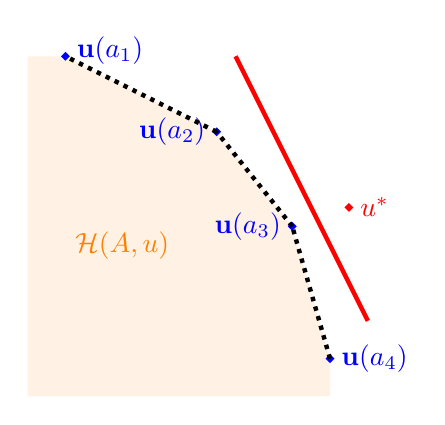
\begin{tikzpicture}[domain=0:3, scale=4.8, ultra thick]    
	
%   \fill[orange!15] (0,0)--(1,0)--(1,0.3)--(0.8,0.7)--(0.4,1.1)--(0,1.1)--(0,0);
    \fill[orange!10] (0.2,0.1)--(1,0.1)--(1,0.2)--(0.9,0.55)--(0.7,0.8)--(0.3,1)--(0.2,1)--(0.2,0.1);
    
%	\draw[<->] (0,1.1) node[left]{$\theta=2$} -- (0,0)-- (1.2,0) node[below,xshift=-5]{$\theta=1$};
	
   
    
    \filldraw[blue] (1,0.2)circle (0.1pt)node[right]{$\bu(a_4)$};
    \filldraw[blue] (0.9,0.55)circle (0.1pt)node[left]{$\bu(a_3)$};
    \filldraw[blue] (0.7,0.8)circle (0.1pt)node[left]{$\bu(a_2)$};
    \filldraw[blue] (0.3,1)circle (0.1pt)node[right,yshift=2]{$\bu(a_1)$};
    
    \filldraw[red] (1.05,0.6)circle (0.1pt)node[right]{$u^*$};
    
    \draw[red] (1.1,0.3)--(0.75,1) ;
    
	\draw[dotted] (1,0.2)--(0.9,0.55);
	\draw[dotted] (0.9,0.55)--(0.7,0.8);
	\draw[dotted] (0.7,0.8)--(0.3,1);

    \draw[orange] (0.45,0.5)node{$\po(A,u)$};
	
	\end{tikzpicture}   
	\caption{}
   \label{}
\end{figure}


Given the canonical decomposition, for any $\ell' > \ell$,
\[
\lambda \cdot u_\ell^*(1, \cdot)  \leq  \lambda \cdot u_\ell^*(0, \cdot) \Longrightarrow \lambda \cdot u_{\ell'}^*(1,\cdot) < \lambda \cdot u_{\ell'}^*(0, \cdot).
\]
Let $\ell^* = \min\left\{ \ell : \lambda \cdot u_\ell(1, \cdot) \leq 0 \right\},$
where we use the convention that $\min \emptyset = n$.  Then 
\begin{align*}
\lambda \cdot u(a_{\ell^*}, \cdot)  - \lambda \cdot u^* &= \sum_{\ell =1}^{\ell^* - 1} \lambda \cdot u_\ell^*(1) -  \sum_{\ell = 1}^{n- 1} \lambda \cdot u_\ell^*(a_\ell^*) \\
&= \sum_{\ell =1}^{\ell^* - 1} \lambda \cdot (u_\ell^*(1) - u_\ell^*(a_\ell^*)) + \sum_{\ell = \ell^*}^{n- 1} \lambda \cdot (u_\ell^*(0) - u_\ell^*(a_\ell^*)) \geq 0.
\end{align*}
But $u(a_{\ell^*}, \cdot) \in \mathcal{H}(A, u)$, which contradicts Inequality~(\ref{eqn:sep}).

It remains to show that $(A_1^*, u_1^*), \ldots , (A_{n- 1}^*, u_{n -1}^*)$ is an exact decomposition, but this is straightforward since it suffices to show that $\left\{u(a, \cdot): a \in A\right\} \subseteq \mathcal{H}\left(\bigoplus_{\ell = 1}^{n- 1} (A_{\ell}^*, u_\ell^*) \right)$.
Clearly this is the case since for every action $a_k \in A$, $u(a_k) = \sum_{\ell = 1}^{k - 1} u_\ell^*(1).$
\end{proof}



\subsection{Proof of \autoref{thm:weakde}}\label{proof:weakde}
We start from proving the following lemma that will be useful in the proof.
\begin{lem}\label{lem:weakde}
If $(A_\ell,u_\ell)_{\ell=1}^k$ is a weak decomposition of $(A,u)$,
\[V(P_1, \ldots , P_m; (A,u)) \geq \sum_{\ell = 1}^{k} V(P_1,...,P_m; (A_\ell,u_\ell)).\]
\end{lem}
\begin{proof}

Suppose $P^*$ is a solution to 
\[\min_{P\in\mathcal{P}(P_1,...,P_m)}\max_{\sigma:\mathbf{Y}\rightarrow \Delta A}\sum_{\theta \in \Theta} \sum_{\mathbf{y} \in \mathbf{Y}} P(\mathbf{y} \mid \theta) u\left(\theta,\sigma(\mathbf{y})\right).\]
From minmax theorem, 
\[V(P_1, \ldots , P_m; (A,u))=\max_{\sigma:\mathbf{Y}\rightarrow \Delta A}\sum_{\theta \in \Theta} \sum_{\mathbf{y} \in \mathbf{Y}} P^*(\mathbf{y} \mid \theta) u\left(\theta,\sigma(\mathbf{y})\right).\]
For $\ell=1,...,k$, define $\sigma_\ell^*$ be a solution to 
\[\max_{\sigma_\ell:\mathbf{Y}\rightarrow \Delta A_\ell}\sum_{\theta \in \Theta} \sum_{\mathbf{y} \in \mathbf{Y}} P^*(\mathbf{y} \mid \theta) u_\ell(\theta,\sigma_\ell(y)).\]

Now we have
\begin{equation}\label{eq:weakdevalue}
\begin{aligned}
    \sum_{\ell = 1}^{k} V(P_1,...,P_m; (A_\ell,u_\ell))&=\sum_{\ell = 1}^{k} \max_{\sigma_\ell:\mathbf{Y}\rightarrow \Delta A_\ell} \min_{P\in\mathcal{P}(P_1,...,P_m)}\sum_{\theta \in \Theta} \sum_{\mathbf{y} \in \mathbf{Y}} P(\mathbf{y} \mid \theta) u_\ell\left(\theta,\sigma_\ell(\mathbf{y})\right)\\
    &\leq\sum_{\ell = 1}^{k} \max_{\sigma_\ell:\mathbf{Y}\rightarrow \Delta A_\ell} \sum_{\theta \in \Theta} \sum_{\mathbf{y} \in \mathbf{Y}} P^*(\mathbf{y} \mid \theta) u_\ell\left(\theta,\sigma_\ell(\mathbf{y})\right)\\
    &= \sum_{\ell = 1}^{k}  \sum_{\theta \in \Theta} \sum_{\mathbf{y} \in \mathbf{Y}} P^*(\mathbf{y} \mid \theta) u_\ell\left(\theta,\sigma_\ell^*(\mathbf{y})\right)
\end{aligned}
\end{equation}
From the definition of weak decomposition, there exists $\hat{\sigma}:\mathbf{Y}\rightarrow A$ such that $u(\theta,\hat{\sigma}(\mathbf{y}))\geq \sum_{\ell=1}^k u_\ell(\theta,\sigma^*_\ell(\mathbf{y}))$ for all $\mathbf{y}$ and $\theta.$

Therefore,
\begin{equation}\label{eq:weakdevalue2}
\begin{aligned}
    \sum_{\ell = 1}^{k}  \sum_{\theta \in \Theta} \sum_{\mathbf{y} \in \mathbf{Y}} P^*(\mathbf{y} \mid \theta) u_\ell\left(\theta,\sigma_\ell^*(\mathbf{y})\right)&= \sum_{\theta \in \Theta} \sum_{\mathbf{y} \in \mathbf{Y}} P^*(\mathbf{y} \mid \theta)  \sum_{\ell = 1}^{k} u_\ell\left(\theta,\sigma_\ell^*(\mathbf{y})\right)\\
    &\leq \sum_{\theta \in \Theta} \sum_{\mathbf{y} \in \mathbf{Y}} P^*(\mathbf{y} \mid \theta)u(\theta,\hat{\sigma}(\mathbf{y}))\\
    &\leq \max_{\sigma:\mathbf{Y}\rightarrow \Delta A}\sum_{\theta \in \Theta} \sum_{\mathbf{y} \in \mathbf{Y}} P^*(\mathbf{y} \mid \theta)u(\theta,\sigma(\mathbf{y}))\\
    &=V(P_1,...,P_m;(A,u))
\end{aligned}
\end{equation}
The statement of the lemma follows immediately from \eqref{eq:weakdevalue} and \eqref{eq:weakdevalue2}
\end{proof}

\begin{proof}[Proof of \autoref{thm:weakde}]
Consider a robustly optimal strategy $\sigma^*:\mathbf{Y}\rightarrow \Delta(A)$ so
\[V(P_1,...,P_m;(A,u))=\min _{P \in \mathcal{P}\left(P_{1}, \ldots, P_{m}\right)} \sum_{\theta \in \Theta} \sum_{\mathbf{y} \in \mathbf{Y}} P(\mathbf{y} \mid \theta) u\left(\theta,\sigma^{*}(\mathbf{y})\right).\]
By considering the dual of the above linear program (Kantorovich dual), we obtain:
\begin{align*}
    V\left(P_{1}, \ldots, P_{m},(A, u)\right) & =\max _{\phi_{1}: \Theta\times Y_{1} \rightarrow \mathbb{R}, \ldots, \phi_{m}: \Theta\times Y_{m} \rightarrow \mathbb{R}} \sum_{j=1}^{m} \sum_{\theta \in \Theta} \sum_{y_{j} \in Y_{j}} P_{j}\left(y_{j} \mid \theta\right) \phi_{j}\left( \theta,y_{j}\right)\\
    &\text{s.t. }\sum_{j=1}^{m} \phi_{j}\left(\theta,y_{j}\right) \leq u\left(\theta,\sigma^{*}(\mathbf{y})\right) \text { for all }(\theta, \mathbf{y}) \in \Theta \times \mathbf{Y}
    \addtocounter{equation}{1}\tag{\theequation} \label{eqn:constraint}
\end{align*}

Let $\phi_1^*,...,\phi_m^*$ be the solution to the dual program. Define the collection of decision problems $\{(A_j,u_j)\}_{j=1}^m$ such that $A_j=Y_j$ and $u_j=\phi_j^*$. From the constraint \eqref{eqn:constraint}, $((A_1,u_1),\ldots,(A_m,u_m))$ forms a weak decomposition of $(A,u)$. 

Moreover, in every ``sub-problem'' $(A_j,u_j)$, by playing the strategy 
\[\sigma^j(y_1,...,y_j,...,y_m)=y_j\quad \text{ for all } (y_1,...,y_m),\] 
the agent achieves exactly a payoff of
\begin{align*}
    \sum_{\theta \in \Theta} \sum_{\left(y_{1}, \ldots, y_{m}\right) \in \mathbf{Y}} P(y_{1}, \ldots, y_{m} \mid \theta) u_j(\theta, \sigma^j(y_{1}, \ldots, y_{m}))
    =&\sum_{\theta \in \Theta} \sum_{y_j \in Y_j} P_j(y_j \mid \theta) u_j(\theta, \sigma^j(y_{1}, \ldots, y_{m}))\\
    =&\sum_{\theta \in \Theta} \sum_{y_j \in Y_j} P_j(y_j \mid \theta) \phi_j^*(\theta, y_j),
\end{align*}
which implies $V(P_1,...,P_m;(A_j,u_j))\geq \max\limits_{\ell=1,...,m} V(P_\ell;(A_j,u_j))\geq \sum_{\theta \in \Theta} \sum_{y_j \in Y_j} P_j(y_j|\theta) \phi_j^*(\theta, y_j)$. 

Summing over all $j=1,...,m$ we have 
\begin{equation}\label{eq:weakde}
    \sum_{j=1}^m V(P_1,...,P_m;(A_j,u_j))\geq \sum_{j=1}^m\max_{\ell=1,...,m} V(P_\ell;(A_j,u_j)) \geq \sum_{j=1}^m \sum_{\theta \in \Theta} \sum_{y_j \in Y_j} P_j(y_j \mid \theta) \phi_j^*(\theta, y_j).
\end{equation}

Now from \autoref{lem:weakde}, equation \eqref{eq:weakde}, and $\{\phi_j^*\}_{j=1}^m$ being the solution to the dual program, we have
\begin{align*}
    V(P_1, \ldots , P_m; (A,u))&\geq \sum_{j=1}^{m} V(P_1,...,P_m; (A_j,u_j))\\
    &\geq \sum_{j=1}^m\max_{\ell=1,...,m} V(P_\ell;(A_j,u_j))\\
    &\geq \sum_{j=1}^{m}\sum_{\theta\in\Theta}\sum_{y_j \in Y_j} P_j(y_j \mid \theta) \phi_j^*(\theta, y_j)\\
    &= V(P_1, \ldots , P_m; (A,u))
\end{align*}
which implies $V(P_1, \ldots , P_m; (A,u))=\sum_{j=1}^m\max_{\ell=1,...,m} V(P_\ell;(A_j,u_j))$.





\end{proof}

\end{document}